\documentclass[11pt]{amsart}
%\documentclass[11pt]{report}
\usepackage[toc,page]{appendix}
\usepackage{float}
\usepackage{mathtools}
\usepackage{geometry}        % See geometry.pdf to learn the layout options.
\geometry{a4paper}           % ... or a4paper or a5paper or ...
%\geometry{landscape}        % Activate for for rotated page geometry
%\usepackage[parfill]{parskip} % Activate to begin paragraphs with empty line
\usepackage{graphicx}
\usepackage{amssymb}
\usepackage{epstopdf}
\usepackage{longtable}

\usepackage[most]{tcolorbox}
\definecolor{block-gray}{gray}{0.85}
\newtcolorbox{myquote}{colback=block-gray,grow to right by=+0mm,grow to left by=-10mm, boxrule=0pt,boxsep=0pt,breakable}

\DeclareGraphicsRule{.tif}{png}{.png}{`convert #1 `dirname #1`/`basename #1 .tif`.png}
\graphicspath{ {images/} }

\renewcommand{\familydefault}{\sfdefault}
\newcounter{defctr}

\title{Naigama parsing system (Compendium)}
\author{Kees-Jan Hermans}
%\date{}                     % Activate to display a given date or no date

\begin{document}
\maketitle

This document contains a description of Naigama, a software
implementation of a Parsing Expression Grammar compiler,
assembler, and bytecode execution engine.

\vspace*{3\baselineskip}

\begin{figure}[H]
\centering
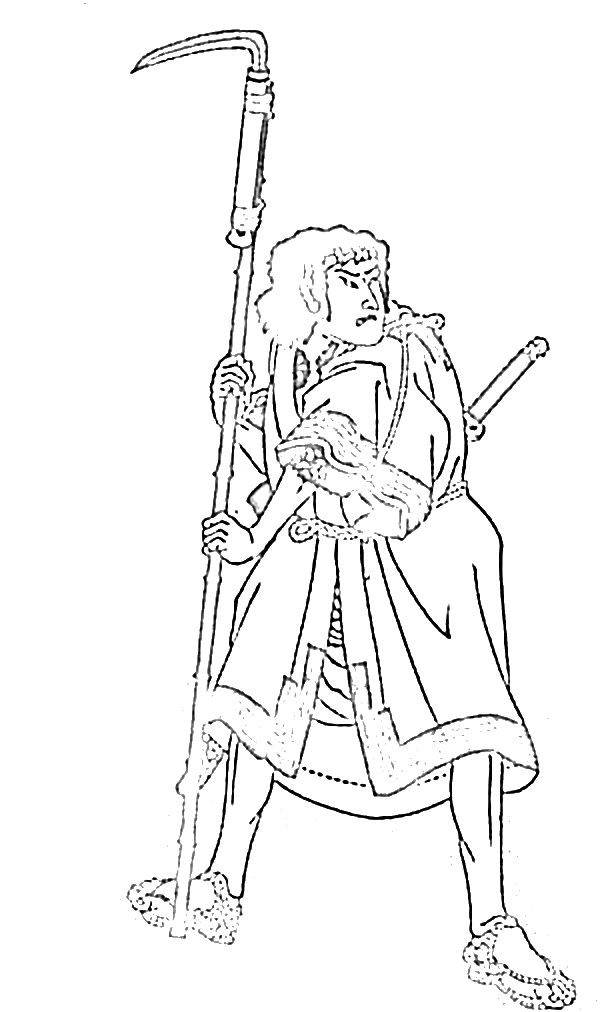
\includegraphics[width=60mm]{naigama}
\end{figure}

\vfill

\begin{table}[]
\centering
\begin{tabular}{ll}
Accompanies release & \input{../../../release} \\
Author &  Kees-Jan Hermans / kees.jan.hermans@gmail.com \\
Classification & - \\
Generated on & \today \\
\end{tabular}
\end{table}

% Accompanies release: \input{../../release}
% 
% Author: Kees-Jan Hermans / kees.jan.hermans@gmail.com
% 
% Classification: -
% 
% Generated on: \today
\newpage

\tableofcontents

\setlength{\parindent}{4em}
\setlength{\parskip}{1em}

\newpage
\section{Colofon}

\listoftables

\newpage

\newpage
\begin{appendices}

\section{Instructions}
\label{app:instr}

This appendix treats all Naigama (assembly / bytecode) instructions,
plus the FAIL event (which eats up the execution stack up to and
including the highest 'catch' element).


%DEADBEEF
\newpage
\subsection{Instruction: any}

\subsubsection{Summary}

The 'any' instruction checks to see if there is a character of input
left to consume, and consumes it if there is. Otherwise it causes a failure.

\subsubsection{Grammar and Compiling}

The '.' (dot) matcher used in grammar, like in regular expressions
\cite{bib:regex}, means 'match any character'. In Perl \cite{bib:perl}
a modifier has to be added to make it include matching of newlines.
In Naigama, 'any character' is confined to 8-bit characters (bytes).

\subsubsection{Assembly Syntax}

\begin{myquote}
\begin{verbatim}
ANYINSTR <- 'any'

\end{verbatim}
\end{myquote}

\subsubsection{Bytecode Encoding}

This instruction is structured in bytecode as follows:

%DEADBEEF
$_0$\ 
\fbox{%
  \parbox{20pt}{%
00
  }%
}
\fbox{%
  \parbox{20pt}{%
00
  }%
}
\fbox{%
  \parbox{20pt}{%
03
  }%
}
\fbox{%
  \parbox{20pt}{%
21
  }%
}

%DEADBEEF
\subsubsection{Execution State Change}

.

Original state: \textit{(p, i, e, c)}

Operation: \textbf{any} ; i \ \textless \ $\vert$S$\vert$

Failure state: \textit{(\textbf{Fail}, i, e, c)}

Success state: \textit{(p + 1, i + 1, e, c)}



\newpage
\subsection{Instruction: backcommit}

\subsubsection{Mode}
This instruction is available in mode 0 (parser).
\subsubsection{Summary}

\InputIfFileExists{instr_backcommit_summary.tex}{}{}

\subsubsection{Grammar and Compiling}

\InputIfFileExists{instr_backcommit_compiling.tex}{}{}

\subsubsection{Assembly Syntax}

\begin{myquote}
\begin{verbatim}
BACKCOMMITINSTR <- { 'backcommit' } S LABEL
S <- %s+
LABEL <- { [a-zA-Z0-9_]^1-64 }
\end{verbatim}
\end{myquote}

\subsubsection{Bytecode Encoding}

This instruction has a size of 8 bytes and is structured in bytecode as follows:

%DEADBEEF
$_{00}$\ 
\fbox{%
  \parbox{20pt}{%
00
  }%
}
\fbox{%
  \parbox{20pt}{%
04
  }%
}
\fbox{%
  \parbox{20pt}{%
03
  }%
}
\fbox{%
  \parbox{20pt}{%
c0
  }%
}



$_{04}$\ 
\fbox{%
  \parbox{20pt}{%
00
  }%
}
\fbox{%
  \parbox{20pt}{%
00
  }%
}
\fbox{%
  \parbox{20pt}{%
00
  }%
}
\fbox{%
  \parbox{20pt}{%
00
  }%
}

%DEADBEEF
\subsubsection{Execution State Change}

.

\InputIfFileExists{instr_backcommit_state.tex}{}{}



\newpage
\subsection{Instruction: call}

\subsubsection{Mode}
This instruction is available in mode 0 (parser).
\subsubsection{Summary}

\InputIfFileExists{instr_call_summary.tex}{}{}

\subsubsection{Grammar and Compiling}

\InputIfFileExists{instr_call_compiling.tex}{}{}

\subsubsection{Assembly Syntax}

\begin{myquote}
\begin{verbatim}
CALLINSTR <- { 'call' } S LABEL
S <- %s+
LABEL <- { [a-zA-Z0-9_]^1-64 }
\end{verbatim}
\end{myquote}

\subsubsection{Bytecode Encoding}

This instruction has a size of 8 bytes and is structured in bytecode as follows:

%DEADBEEF
$_{00}$\ 
\fbox{%
  \parbox{20pt}{%
00
  }%
}
\fbox{%
  \parbox{20pt}{%
04
  }%
}
\fbox{%
  \parbox{20pt}{%
03
  }%
}
\fbox{%
  \parbox{20pt}{%
82
  }%
}



$_{04}$\ 
\fbox{%
  \parbox{20pt}{%
00
  }%
}
\fbox{%
  \parbox{20pt}{%
00
  }%
}
\fbox{%
  \parbox{20pt}{%
00
  }%
}
\fbox{%
  \parbox{20pt}{%
00
  }%
}

%DEADBEEF
\subsubsection{Execution State Change}

.

\InputIfFileExists{instr_call_state.tex}{}{}



\newpage
\subsection{Instruction: catch}

\subsubsection{Summary}

The 'catch' instruction pushes a 'catch' element on the stack,
in which the current state of the engine is captured (input position,
height of the action list), as well as a bytecode offset, which
is where the engine jumps to when the element is popped due to a FAIL
condition.

\subsubsection{Grammar and Compiling}

Several constructs in the Naigama grammar emit a 'catch' instruction,
for example:

\begin{itemize}

\item A 'choice' situation, which is when an OR operator ('/', or
slash forward) is introduced in an expression.

\item A 'not' situation, which is when a matcher is prefixed with a NOT
operator ('!', or exclamation mark).

\item A 'not-not' situation, which is when a matcher is prefixed with an
ampersand ('\&').

\item A quantifier on a matcher that is forgiving, for example allowing
infinite repetitions of a matcher, or values between a minimum and a
maximum.

\end{itemize}

\subsubsection{Assembly Syntax}

\begin{myquote}
\begin{verbatim}
CATCHINSTR <- 'catch' S LABEL
S          <- %s+
LABEL      <- [a-zA-Z0-9_]^1-64

\end{verbatim}
\end{myquote}

\subsubsection{Bytecode Encoding}

This instruction is structured in bytecode as follows:

%DEADBEEF
$_0$\ 
\fbox{%
  \parbox{20pt}{%
00
  }%
}
\fbox{%
  \parbox{20pt}{%
04
  }%
}
\fbox{%
  \parbox{20pt}{%
0a
  }%
}
\fbox{%
  \parbox{20pt}{%
03
  }%
}

%DEADBEEF

$_4$\
\fbox{%
  \parbox{20pt}{%
nn
  }%
}
\fbox{%
  \parbox{20pt}{%
nn
  }%
}
\fbox{%
  \parbox{20pt}{%
nn
  }%
}
\fbox{%
  \parbox{20pt}{%
nn
  }%
}

Where 'nn' is a 32-bit, network encoded, valid bytecode offset.

\subsubsection{Execution State Change}

.

Original state: \textit{(p, i, e, c)}

Operation: \textbf{catch n}

Failure state: -

Success state: \textit{(p + 1, i, e:(n,p,i), c)}



\newpage
\subsection{Instruction: char}

\subsubsection{Summary}

The 'char' instruction compares its only parameter, a character value,
against the character value at the current input offset. If they are
equal, the match is considered a success, and the engine moves to the
next instruction. If they are not equal, the FAIL condition is raised.

\subsubsection{Grammar and Compiling}

In grammar, the 'char' instruction is emitted by the compiler from
the treatment of a string literal.

\subsubsection{Assembly Syntax}

\begin{myquote}
\begin{verbatim}
CHARINSTR <- 'char' S HEXBYTE
S         <- %s+
HEXBYTE   <- [0-9a-fA-F]^2

\end{verbatim}
\end{myquote}
\subsubsection{Bytecode Encoding}

This instruction is structured in bytecode as follows:

%DEADBEEF
$_0$\ 
\fbox{%
  \parbox{20pt}{%
00
  }%
}
\fbox{%
  \parbox{20pt}{%
04
  }%
}
\fbox{%
  \parbox{20pt}{%
05
  }%
}
\fbox{%
  \parbox{20pt}{%
09
  }%
}

%DEADBEEF

$_4$\
\fbox{%
  \parbox{20pt}{%
nn
  }%
}
\fbox{%
  \parbox{20pt}{%
nn
  }%
}
\fbox{%
  \parbox{20pt}{%
nn
  }%
}
\fbox{%
  \parbox{20pt}{%
nn
  }%
}

Where 'nn' is a 32-bit, network encoded, character value.

\subsubsection{Execution State Change}

.

Original state: \textit{(p, i, e, c)}

Operation: \textbf{char c}

Failure state: \textit{(\textbf{Fail}, i, e, c)}

Success state: \textit{(p + 1, i + 1, e, c)}



\newpage
\subsection{Instruction: closecapture}

\subsubsection{Mode}
This instruction is available in mode 0 (parser).
\subsubsection{Summary}

\InputIfFileExists{instr_closecapture_summary.tex}{}{}

\subsubsection{Grammar and Compiling}

\InputIfFileExists{instr_closecapture_compiling.tex}{}{}

\subsubsection{Assembly Syntax}

\begin{myquote}
\begin{verbatim}
CLOSECAPTUREINSTR <- { 'closecapture' } S SLOT ( S TYPE )?
S <- %s+
SLOT <- UNSIGNED
TYPE <- UNSIGNED
\end{verbatim}
\end{myquote}

\subsubsection{Bytecode Encoding}

This instruction has a size of 8 bytes and is structured in bytecode as follows:

%DEADBEEF
$_{00}$\ 
\fbox{%
  \parbox{20pt}{%
00
  }%
}
\fbox{%
  \parbox{20pt}{%
04
  }%
}
\fbox{%
  \parbox{20pt}{%
03
  }%
}
\fbox{%
  \parbox{20pt}{%
00
  }%
}



$_{04}$\ 
\fbox{%
  \parbox{20pt}{%
00
  }%
}
\fbox{%
  \parbox{20pt}{%
00
  }%
}
\fbox{%
  \parbox{20pt}{%
00
  }%
}
\fbox{%
  \parbox{20pt}{%
00
  }%
}

%DEADBEEF
\subsubsection{Execution State Change}

.

\InputIfFileExists{instr_closecapture_state.tex}{}{}



\newpage
\subsection{Instruction: commit}

\subsubsection{Summary}

\InputIfFileExists{instr_commit_summary.tex}{}{}

\subsubsection{Grammar and Compiling}

\InputIfFileExists{instr_commit_compiling.tex}{}{}

\subsubsection{Assembly Syntax}

\begin{myquote}
\begin{verbatim}
COMMITINSTR <- { 'commit' } S LABEL
S <- %s+
LABEL <- { [a-zA-Z0-9_]^1-256 }
\end{verbatim}
\end{myquote}

\subsubsection{Bytecode Encoding}

This instruction has a size of 8 bytes and is structured in bytecode as follows:

%DEADBEEF
$_{00}$\ 
\fbox{%
  \parbox{20pt}{%
00
  }%
}
\fbox{%
  \parbox{20pt}{%
04
  }%
}
\fbox{%
  \parbox{20pt}{%
03
  }%
}
\fbox{%
  \parbox{20pt}{%
36
  }%
}



$_{04}$\ 
\fbox{%
  \parbox{20pt}{%
00
  }%
}
\fbox{%
  \parbox{20pt}{%
00
  }%
}
\fbox{%
  \parbox{20pt}{%
00
  }%
}
\fbox{%
  \parbox{20pt}{%
00
  }%
}

%DEADBEEF
\InputIfFileExists{instr_commit_bytecode.tex}{}{}

\subsubsection{Execution State Change}

.

\InputIfFileExists{instr_commit_state.tex}{}{}



\newpage
\subsection{Instruction: condjump}

\subsubsection{Summary}

\InputIfFileExists{instr_condjump_summary.tex}{}{}

\subsubsection{Grammar and Compiling}

\InputIfFileExists{instr_condjump_compiling.tex}{}{}

\subsubsection{Assembly Syntax}

\begin{myquote}
\begin{verbatim}
CONDJUMPINSTR <- { 'condjump' } S REGISTER S LABEL
S <- %s+
REGISTER <- UNSIGNED
LABEL <- { [a-zA-Z0-9_]^1-64 }
\end{verbatim}
\end{myquote}

\InputIfFileExists{instr_condjump_assembly.tex}{}{}

\subsubsection{Bytecode Encoding}

This instruction has a size of 12 bytes and is structured in bytecode as follows:

%DEADBEEF
$_{00}$\ 
\fbox{%
  \parbox{20pt}{%
00
  }%
}
\fbox{%
  \parbox{20pt}{%
08
  }%
}
\fbox{%
  \parbox{20pt}{%
03
  }%
}
\fbox{%
  \parbox{20pt}{%
21
  }%
}



$_{04}$\ 
\fbox{%
  \parbox{20pt}{%
00
  }%
}
\fbox{%
  \parbox{20pt}{%
00
  }%
}
\fbox{%
  \parbox{20pt}{%
00
  }%
}
\fbox{%
  \parbox{20pt}{%
00
  }%
}



$_{08}$\ 
\fbox{%
  \parbox{20pt}{%
00
  }%
}
\fbox{%
  \parbox{20pt}{%
00
  }%
}
\fbox{%
  \parbox{20pt}{%
00
  }%
}
\fbox{%
  \parbox{20pt}{%
00
  }%
}

%DEADBEEF
\InputIfFileExists{instr_condjump_bytecode.tex}{}{}

\subsubsection{Execution State Change}

.

\InputIfFileExists{instr_condjump_state.tex}{}{}



\newpage
\subsection{Instruction: counter}

\subsubsection{Summary}

\InputIfFileExists{instr_counter_summary.tex}{}{}

\subsubsection{Grammar and Compiling}

\InputIfFileExists{instr_counter_compiling.tex}{}{}

\subsubsection{Assembly Syntax}

\begin{myquote}
\begin{verbatim}
COUNTERINSTR <- { 'counter' } S REGISTER S UNSIGNED
S <- %s+
REGISTER <- UNSIGNED
UNSIGNED <- { [0-9]+ }
\end{verbatim}
\end{myquote}

\subsubsection{Bytecode Encoding}

This instruction has a size of 12 bytes and is structured in bytecode as follows:

%DEADBEEF
$_{00}$\ 
\fbox{%
  \parbox{20pt}{%
00
  }%
}
\fbox{%
  \parbox{20pt}{%
08
  }%
}
\fbox{%
  \parbox{20pt}{%
03
  }%
}
\fbox{%
  \parbox{20pt}{%
56
  }%
}



$_{04}$\ 
\fbox{%
  \parbox{20pt}{%
00
  }%
}
\fbox{%
  \parbox{20pt}{%
00
  }%
}
\fbox{%
  \parbox{20pt}{%
00
  }%
}
\fbox{%
  \parbox{20pt}{%
00
  }%
}



$_{08}$\ 
\fbox{%
  \parbox{20pt}{%
00
  }%
}
\fbox{%
  \parbox{20pt}{%
00
  }%
}
\fbox{%
  \parbox{20pt}{%
00
  }%
}
\fbox{%
  \parbox{20pt}{%
00
  }%
}

%DEADBEEF
\InputIfFileExists{instr_counter_bytecode.tex}{}{}

\subsubsection{Execution State Change}

.

\InputIfFileExists{instr_counter_state.tex}{}{}



\newpage
\subsection{Instruction: end}

\subsubsection{Summary}

\InputIfFileExists{instr_end_summary.tex}{}{}

\subsubsection{Grammar and Compiling}

\InputIfFileExists{instr_end_compiling.tex}{}{}

\subsubsection{Assembly Syntax}

\begin{myquote}
\begin{verbatim}
ENDINSTR <- { 'end' } S CODE
S <- %s+
CODE <- UNSIGNED
\end{verbatim}
\end{myquote}

\InputIfFileExists{instr_end_assembly.tex}{}{}

\subsubsection{Bytecode Encoding}

This instruction has a size of 8 bytes and is structured in bytecode as follows:

%DEADBEEF
$_{00}$\ 
\fbox{%
  \parbox{20pt}{%
00
  }%
}
\fbox{%
  \parbox{20pt}{%
04
  }%
}
\fbox{%
  \parbox{20pt}{%
00
  }%
}
\fbox{%
  \parbox{20pt}{%
d8
  }%
}



$_{04}$\ 
\fbox{%
  \parbox{20pt}{%
00
  }%
}
\fbox{%
  \parbox{20pt}{%
00
  }%
}
\fbox{%
  \parbox{20pt}{%
00
  }%
}
\fbox{%
  \parbox{20pt}{%
00
  }%
}

%DEADBEEF
\InputIfFileExists{instr_end_bytecode.tex}{}{}

\subsubsection{Execution State Change}

.

\InputIfFileExists{instr_end_state.tex}{}{}



\newpage
\subsection{Instruction: endisolate}

\subsubsection{Mode}
This instruction is available in mode 0 (parser).
\subsubsection{Summary}

\InputIfFileExists{instr_endisolate_summary.tex}{}{}

\subsubsection{Grammar and Compiling}

\InputIfFileExists{instr_endisolate_compiling.tex}{}{}

\subsubsection{Assembly Syntax}

\begin{myquote}
\begin{verbatim}
ENDISOLATEINSTR <- { 'endisolate' }
\end{verbatim}
\end{myquote}

\subsubsection{Bytecode Encoding}

This instruction has a size of 4 bytes and is structured in bytecode as follows:

%DEADBEEF
$_{00}$\ 
\fbox{%
  \parbox{20pt}{%
00
  }%
}
\fbox{%
  \parbox{20pt}{%
00
  }%
}
\fbox{%
  \parbox{20pt}{%
30
  }%
}
\fbox{%
  \parbox{20pt}{%
05
  }%
}

%DEADBEEF
\subsubsection{Execution State Change}

.

\InputIfFileExists{instr_endisolate_state.tex}{}{}



\newpage
\subsection{Instruction: endreplace}

\subsubsection{Mode}
This instruction is available in mode 0 (parser).
\subsubsection{Summary}

\InputIfFileExists{instr_endreplace_summary.tex}{}{}

\subsubsection{Grammar and Compiling}

\InputIfFileExists{instr_endreplace_compiling.tex}{}{}

\subsubsection{Assembly Syntax}

\begin{myquote}
\begin{verbatim}
ENDREPLACEINSTR <- { 'endreplace' }
\end{verbatim}
\end{myquote}

\subsubsection{Bytecode Encoding}

This instruction has a size of 4 bytes and is structured in bytecode as follows:

%DEADBEEF
$_{00}$\ 
\fbox{%
  \parbox{20pt}{%
00
  }%
}
\fbox{%
  \parbox{20pt}{%
00
  }%
}
\fbox{%
  \parbox{20pt}{%
03
  }%
}
\fbox{%
  \parbox{20pt}{%
99
  }%
}

%DEADBEEF
\InputIfFileExists{instr_endreplace_bytecode.tex}{}{}

\subsubsection{Execution State Change}

.

\InputIfFileExists{instr_endreplace_state.tex}{}{}



\newpage
\subsection{Instruction: fail}

\subsubsection{Summary}

\InputIfFileExists{instr_fail_summary.tex}{}{}

\subsubsection{Grammar and Compiling}

\InputIfFileExists{instr_fail_compiling.tex}{}{}

\subsubsection{Assembly Syntax}

\begin{myquote}
\begin{verbatim}
FAILINSTR <- { 'fail' }
\end{verbatim}
\end{myquote}

\InputIfFileExists{instr_fail_assembly.tex}{}{}

\subsubsection{Bytecode Encoding}

This instruction has a size of 4 bytes and is structured in bytecode as follows:

%DEADBEEF
$_{00}$\ 
\fbox{%
  \parbox{20pt}{%
00
  }%
}
\fbox{%
  \parbox{20pt}{%
00
  }%
}
\fbox{%
  \parbox{20pt}{%
03
  }%
}
\fbox{%
  \parbox{20pt}{%
4b
  }%
}

%DEADBEEF
\InputIfFileExists{instr_fail_bytecode.tex}{}{}

\subsubsection{Execution State Change}

.

\InputIfFileExists{instr_fail_state.tex}{}{}



\newpage
\subsection{Instruction: failtwice}

\subsubsection{Mode}
This instruction is available in mode 0 (parser).
\subsubsection{Summary}

\InputIfFileExists{instr_failtwice_summary.tex}{}{}

\subsubsection{Grammar and Compiling}

\InputIfFileExists{instr_failtwice_compiling.tex}{}{}

\subsubsection{Assembly Syntax}

\begin{myquote}
\begin{verbatim}
FAILTWICEINSTR <- { 'failtwice' }
\end{verbatim}
\end{myquote}

\subsubsection{Bytecode Encoding}

This instruction has a size of 4 bytes and is structured in bytecode as follows:

%DEADBEEF
$_{00}$\ 
\fbox{%
  \parbox{20pt}{%
00
  }%
}
\fbox{%
  \parbox{20pt}{%
00
  }%
}
\fbox{%
  \parbox{20pt}{%
03
  }%
}
\fbox{%
  \parbox{20pt}{%
90
  }%
}

%DEADBEEF
\subsubsection{Execution State Change}

.

\InputIfFileExists{instr_failtwice_state.tex}{}{}



\newpage
\subsection{Instruction: isolate}

\subsubsection{Summary}

\InputIfFileExists{instr_isolate_summary.tex}{}{}

\subsubsection{Grammar and Compiling}

\InputIfFileExists{instr_isolate_compiling.tex}{}{}

\subsubsection{Assembly Syntax}

\begin{myquote}
\begin{verbatim}
ISOLATEINSTR <- { 'isolate' } S SLOT
S <- %s+
SLOT <- UNSIGNED
\end{verbatim}
\end{myquote}

\InputIfFileExists{instr_isolate_assembly.tex}{}{}

\subsubsection{Bytecode Encoding}

This instruction has a size of 8 bytes and is structured in bytecode as follows:

%DEADBEEF
$_{00}$\ 
\fbox{%
  \parbox{20pt}{%
00
  }%
}
\fbox{%
  \parbox{20pt}{%
04
  }%
}
\fbox{%
  \parbox{20pt}{%
30
  }%
}
\fbox{%
  \parbox{20pt}{%
03
  }%
}



$_{04}$\ 
\fbox{%
  \parbox{20pt}{%
00
  }%
}
\fbox{%
  \parbox{20pt}{%
00
  }%
}
\fbox{%
  \parbox{20pt}{%
00
  }%
}
\fbox{%
  \parbox{20pt}{%
00
  }%
}

%DEADBEEF
\InputIfFileExists{instr_isolate_bytecode.tex}{}{}

\subsubsection{Execution State Change}

.

\InputIfFileExists{instr_isolate_state.tex}{}{}



\newpage
\subsection{Instruction: jump}

\subsubsection{Mode}
This instruction is available in both mode 0 (parser) and mode 1 (script interpreter).
\subsubsection{Summary}

\InputIfFileExists{instr_jump_summary.tex}{}{}

\subsubsection{Grammar and Compiling}

\InputIfFileExists{instr_jump_compiling.tex}{}{}

\subsubsection{Assembly Syntax}

\begin{myquote}
\begin{verbatim}
JUMPINSTR <- { 'jump' } S LABEL
S <- %s+
LABEL <- { [a-zA-Z0-9_]^1-64 }
\end{verbatim}
\end{myquote}

\subsubsection{Bytecode Encoding}

This instruction has a size of 8 bytes and is structured in bytecode as follows:

%DEADBEEF
$_{00}$\ 
\fbox{%
  \parbox{20pt}{%
00
  }%
}
\fbox{%
  \parbox{20pt}{%
04
  }%
}
\fbox{%
  \parbox{20pt}{%
03
  }%
}
\fbox{%
  \parbox{20pt}{%
33
  }%
}



$_{04}$\ 
\fbox{%
  \parbox{20pt}{%
00
  }%
}
\fbox{%
  \parbox{20pt}{%
00
  }%
}
\fbox{%
  \parbox{20pt}{%
00
  }%
}
\fbox{%
  \parbox{20pt}{%
00
  }%
}

%DEADBEEF
\subsubsection{Execution State Change}

.

\InputIfFileExists{instr_jump_state.tex}{}{}



\newpage
\subsection{Instruction: maskedchar}

\subsubsection{Mode}
This instruction is available in mode 0 (parser).
\subsubsection{Summary}

\InputIfFileExists{instr_maskedchar_summary.tex}{}{}

\subsubsection{Grammar and Compiling}

\InputIfFileExists{instr_maskedchar_compiling.tex}{}{}

\subsubsection{Assembly Syntax}

\begin{myquote}
\begin{verbatim}
MASKEDCHARINSTR <- { 'maskedchar' } S HEXBYTE S HEXBYTE
S <- %s+
HEXBYTE <- { [0-9a-fA-F]^2 }
\end{verbatim}
\end{myquote}

\subsubsection{Bytecode Encoding}

This instruction has a size of 12 bytes and is structured in bytecode as follows:

%DEADBEEF
$_{00}$\ 
\fbox{%
  \parbox{20pt}{%
00
  }%
}
\fbox{%
  \parbox{20pt}{%
08
  }%
}
\fbox{%
  \parbox{20pt}{%
03
  }%
}
\fbox{%
  \parbox{20pt}{%
65
  }%
}



$_{04}$\ 
\fbox{%
  \parbox{20pt}{%
00
  }%
}
\fbox{%
  \parbox{20pt}{%
00
  }%
}
\fbox{%
  \parbox{20pt}{%
00
  }%
}
\fbox{%
  \parbox{20pt}{%
00
  }%
}



$_{08}$\ 
\fbox{%
  \parbox{20pt}{%
00
  }%
}
\fbox{%
  \parbox{20pt}{%
00
  }%
}
\fbox{%
  \parbox{20pt}{%
00
  }%
}
\fbox{%
  \parbox{20pt}{%
00
  }%
}

%DEADBEEF
\InputIfFileExists{instr_maskedchar_bytecode.tex}{}{}

\subsubsection{Execution State Change}

.

\InputIfFileExists{instr_maskedchar_state.tex}{}{}



\newpage
\subsection{Instruction: mode}

\subsubsection{Mode}
This instruction is available in both mode 0 (parser) and mode 1 (script interpreter).
\subsubsection{Summary}

\InputIfFileExists{instr_mode_summary.tex}{}{}

\subsubsection{Grammar and Compiling}

\InputIfFileExists{instr_mode_compiling.tex}{}{}

\subsubsection{Assembly Syntax}

\begin{myquote}
\begin{verbatim}
MODEINSTR <- { 'mode' } S NUMBER
S <- %s+
NUMBER <- { '-'? [0-9]+ }
\end{verbatim}
\end{myquote}

\subsubsection{Bytecode Encoding}

This instruction has a size of 8 bytes and is structured in bytecode as follows:

%DEADBEEF
$_{00}$\ 
\fbox{%
  \parbox{20pt}{%
00
  }%
}
\fbox{%
  \parbox{20pt}{%
04
  }%
}
\fbox{%
  \parbox{20pt}{%
00
  }%
}
\fbox{%
  \parbox{20pt}{%
0a
  }%
}



$_{04}$\ 
\fbox{%
  \parbox{20pt}{%
00
  }%
}
\fbox{%
  \parbox{20pt}{%
00
  }%
}
\fbox{%
  \parbox{20pt}{%
00
  }%
}
\fbox{%
  \parbox{20pt}{%
00
  }%
}

%DEADBEEF
\subsubsection{Execution State Change}

.

\InputIfFileExists{instr_mode_state.tex}{}{}



\newpage
\subsection{Instruction: noop}

\subsubsection{Mode}
This instruction is available in both mode 0 (parser) and mode 1 (script interpreter).
\subsubsection{Summary}

\InputIfFileExists{instr_noop_summary.tex}{}{}

\subsubsection{Grammar and Compiling}

\InputIfFileExists{instr_noop_compiling.tex}{}{}

\subsubsection{Assembly Syntax}

\begin{myquote}
\begin{verbatim}
NOOPINSTR <- { 'noop' }
\end{verbatim}
\end{myquote}

\subsubsection{Bytecode Encoding}

This instruction has a size of 4 bytes and is structured in bytecode as follows:

%DEADBEEF
$_{00}$\ 
\fbox{%
  \parbox{20pt}{%
00
  }%
}
\fbox{%
  \parbox{20pt}{%
00
  }%
}
\fbox{%
  \parbox{20pt}{%
00
  }%
}
\fbox{%
  \parbox{20pt}{%
00
  }%
}

%DEADBEEF
\InputIfFileExists{instr_noop_bytecode.tex}{}{}

\subsubsection{Execution State Change}

.

\InputIfFileExists{instr_noop_state.tex}{}{}



\newpage
\subsection{Instruction: opencapture}

\subsubsection{Mode}
This instruction is available in mode 0 (parser).
\subsubsection{Summary}

\InputIfFileExists{instr_opencapture_summary.tex}{}{}

\subsubsection{Grammar and Compiling}

\InputIfFileExists{instr_opencapture_compiling.tex}{}{}

\subsubsection{Assembly Syntax}

\begin{myquote}
\begin{verbatim}
OPENCAPTUREINSTR <- { 'opencapture' } S SLOT
S <- %s+
SLOT <- UNSIGNED
\end{verbatim}
\end{myquote}

\subsubsection{Bytecode Encoding}

This instruction has a size of 8 bytes and is structured in bytecode as follows:

%DEADBEEF
$_{00}$\ 
\fbox{%
  \parbox{20pt}{%
00
  }%
}
\fbox{%
  \parbox{20pt}{%
04
  }%
}
\fbox{%
  \parbox{20pt}{%
03
  }%
}
\fbox{%
  \parbox{20pt}{%
9c
  }%
}



$_{04}$\ 
\fbox{%
  \parbox{20pt}{%
00
  }%
}
\fbox{%
  \parbox{20pt}{%
00
  }%
}
\fbox{%
  \parbox{20pt}{%
00
  }%
}
\fbox{%
  \parbox{20pt}{%
00
  }%
}

%DEADBEEF
\subsubsection{Execution State Change}

.

\InputIfFileExists{instr_opencapture_state.tex}{}{}



\newpage
\subsection{Instruction: partialcommit}

\subsubsection{Summary}

\InputIfFileExists{instr_partialcommit_summary.tex}{}{}

\subsubsection{Grammar and Compiling}

\InputIfFileExists{instr_partialcommit_compiling.tex}{}{}

\subsubsection{Assembly Syntax}

\begin{myquote}
\begin{verbatim}
PARTIALCOMMITINSTR <- { 'partialcommit' } S LABEL
S <- %s+
LABEL <- { [a-zA-Z0-9_]^1-256 }
\end{verbatim}
\end{myquote}

\subsubsection{Bytecode Encoding}

This instruction has a size of 8 bytes and is structured in bytecode as follows:

%DEADBEEF
$_{00}$\ 
\fbox{%
  \parbox{20pt}{%
00
  }%
}
\fbox{%
  \parbox{20pt}{%
04
  }%
}
\fbox{%
  \parbox{20pt}{%
03
  }%
}
\fbox{%
  \parbox{20pt}{%
b4
  }%
}



$_{04}$\ 
\fbox{%
  \parbox{20pt}{%
00
  }%
}
\fbox{%
  \parbox{20pt}{%
00
  }%
}
\fbox{%
  \parbox{20pt}{%
00
  }%
}
\fbox{%
  \parbox{20pt}{%
00
  }%
}

%DEADBEEF
\InputIfFileExists{instr_partialcommit_bytecode.tex}{}{}

\subsubsection{Execution State Change}

.

\InputIfFileExists{instr_partialcommit_state.tex}{}{}



\newpage
\subsection{Instruction: quad}

\subsubsection{Summary}

\subsubsection{Grammar and Compiling}

\subsubsection{Assembly Syntax}

\begin{myquote}
\begin{verbatim}

\end{verbatim}
\end{myquote}
\subsubsection{Bytecode Encoding}

This instruction is structured in bytecode as follows:

%DEADBEEF
$_0$\ 
\fbox{%
  \parbox{20pt}{%
00
  }%
}
\fbox{%
  \parbox{20pt}{%
04
  }%
}
\fbox{%
  \parbox{20pt}{%
03
  }%
}
\fbox{%
  \parbox{20pt}{%
09
  }%
}

%DEADBEEF
\subsubsection{Execution State Change}

.

Original state: \textit{(p, i, e, c)}

Operation: \textbf{any} ; i \ \textless \ $\vert$S$\vert$

Failure state: \textit{(\textbf{Fail}, i, e, c)}

Success state: \textit{(p + 1, i + 1, e, c)}



\newpage
\subsection{Instruction: range}

\subsubsection{Mode}
This instruction is available in mode 0 (parser).
\subsubsection{Summary}

\InputIfFileExists{instr_range_summary.tex}{}{}

\subsubsection{Grammar and Compiling}

\InputIfFileExists{instr_range_compiling.tex}{}{}

\subsubsection{Assembly Syntax}

\begin{myquote}
\begin{verbatim}
RANGEINSTR <- { 'range' } S UNSIGNED S UNSIGNED
S <- %s+
UNSIGNED <- { [0-9]+ }
\end{verbatim}
\end{myquote}

\subsubsection{Bytecode Encoding}

This instruction has a size of 12 bytes and is structured in bytecode as follows:

%DEADBEEF
$_{00}$\ 
\fbox{%
  \parbox{20pt}{%
00
  }%
}
\fbox{%
  \parbox{20pt}{%
08
  }%
}
\fbox{%
  \parbox{20pt}{%
03
  }%
}
\fbox{%
  \parbox{20pt}{%
bd
  }%
}



$_{04}$\ 
\fbox{%
  \parbox{20pt}{%
00
  }%
}
\fbox{%
  \parbox{20pt}{%
00
  }%
}
\fbox{%
  \parbox{20pt}{%
00
  }%
}
\fbox{%
  \parbox{20pt}{%
00
  }%
}



$_{08}$\ 
\fbox{%
  \parbox{20pt}{%
00
  }%
}
\fbox{%
  \parbox{20pt}{%
00
  }%
}
\fbox{%
  \parbox{20pt}{%
00
  }%
}
\fbox{%
  \parbox{20pt}{%
00
  }%
}

%DEADBEEF
\subsubsection{Execution State Change}

.

\InputIfFileExists{instr_range_state.tex}{}{}



\newpage
\subsection{Instruction: replace}

\subsubsection{Mode}
This instruction is available in mode 0 (parser).
\subsubsection{Summary}

\InputIfFileExists{instr_replace_summary.tex}{}{}

\subsubsection{Grammar and Compiling}

\InputIfFileExists{instr_replace_compiling.tex}{}{}

\subsubsection{Assembly Syntax}

\begin{myquote}
\begin{verbatim}
REPLACEINSTR <- { 'replace' } S SLOT S LABEL
S <- %s+
SLOT <- UNSIGNED
LABEL <- { [a-zA-Z0-9_]^1-64 }
\end{verbatim}
\end{myquote}

\subsubsection{Bytecode Encoding}

This instruction has a size of 12 bytes and is structured in bytecode as follows:

%DEADBEEF
$_{00}$\ 
\fbox{%
  \parbox{20pt}{%
00
  }%
}
\fbox{%
  \parbox{20pt}{%
08
  }%
}
\fbox{%
  \parbox{20pt}{%
03
  }%
}
\fbox{%
  \parbox{20pt}{%
48
  }%
}



$_{04}$\ 
\fbox{%
  \parbox{20pt}{%
00
  }%
}
\fbox{%
  \parbox{20pt}{%
00
  }%
}
\fbox{%
  \parbox{20pt}{%
00
  }%
}
\fbox{%
  \parbox{20pt}{%
00
  }%
}



$_{08}$\ 
\fbox{%
  \parbox{20pt}{%
00
  }%
}
\fbox{%
  \parbox{20pt}{%
00
  }%
}
\fbox{%
  \parbox{20pt}{%
00
  }%
}
\fbox{%
  \parbox{20pt}{%
00
  }%
}

%DEADBEEF
\InputIfFileExists{instr_replace_bytecode.tex}{}{}

\subsubsection{Execution State Change}

.

\InputIfFileExists{instr_replace_state.tex}{}{}



\newpage
\subsection{Instruction: ret}

\subsubsection{Summary}

\subsubsection{Grammar and Compiling}

\subsubsection{Assembly Syntax}

\begin{myquote}
\begin{verbatim}

\end{verbatim}
\end{myquote}
\subsubsection{Bytecode Encoding}

This instruction is structured in bytecode as follows:

%DEADBEEF
$_0$\ 
\fbox{%
  \parbox{20pt}{%
00
  }%
}
\fbox{%
  \parbox{20pt}{%
00
  }%
}
\fbox{%
  \parbox{20pt}{%
03
  }%
}
\fbox{%
  \parbox{20pt}{%
05
  }%
}

%DEADBEEF
\subsubsection{Execution State Change}

.

Original state: \textit{(p, i, e, c)}

Operation: \textbf{any} ; i \ \textless \ $\vert$S$\vert$

Failure state: \textit{(\textbf{Fail}, i, e, c)}

Success state: \textit{(p + 1, i + 1, e, c)}



\newpage
\subsection{Instruction: scr\_add}

\subsubsection{Mode}
This instruction is available in mode 1 (script interpreter).
\subsubsection{Summary}

\InputIfFileExists{instr_scr_add_summary.tex}{}{}

\subsubsection{Grammar and Compiling}

\InputIfFileExists{instr_scr_add_compiling.tex}{}{}

\subsubsection{Assembly Syntax}

\begin{myquote}
\begin{verbatim}
SCR_ADD <- { 'scr_add' }
\end{verbatim}
\end{myquote}

\subsubsection{Bytecode Encoding}

This instruction has a size of 4 bytes and is structured in bytecode as follows:

%DEADBEEF
$_{00}$\ 
\fbox{%
  \parbox{20pt}{%
00
  }%
}
\fbox{%
  \parbox{20pt}{%
00
  }%
}
\fbox{%
  \parbox{20pt}{%
05
  }%
}
\fbox{%
  \parbox{20pt}{%
0c
  }%
}

%DEADBEEF
\subsubsection{Execution State Change}

.

\InputIfFileExists{instr_scr_add_state.tex}{}{}



\newpage
\subsection{Instruction: scr\_array}

\subsubsection{Mode}
This instruction is available in mode 1 (script interpreter).
\subsubsection{Summary}

\InputIfFileExists{instr_scr_array_summary.tex}{}{}

\subsubsection{Grammar and Compiling}

\InputIfFileExists{instr_scr_array_compiling.tex}{}{}

\subsubsection{Assembly Syntax}

\begin{myquote}
\begin{verbatim}
SCR_ARRAY <- { 'scr_array' } S UNSIGNED
S <- %s+
UNSIGNED <- { [0-9]+ }
\end{verbatim}
\end{myquote}

\subsubsection{Bytecode Encoding}

This instruction has a size of 8 bytes and is structured in bytecode as follows:

%DEADBEEF
$_{00}$\ 
\fbox{%
  \parbox{20pt}{%
00
  }%
}
\fbox{%
  \parbox{20pt}{%
04
  }%
}
\fbox{%
  \parbox{20pt}{%
00
  }%
}
\fbox{%
  \parbox{20pt}{%
06
  }%
}



$_{04}$\ 
\fbox{%
  \parbox{20pt}{%
00
  }%
}
\fbox{%
  \parbox{20pt}{%
00
  }%
}
\fbox{%
  \parbox{20pt}{%
00
  }%
}
\fbox{%
  \parbox{20pt}{%
00
  }%
}

%DEADBEEF
\subsubsection{Execution State Change}

.

\InputIfFileExists{instr_scr_array_state.tex}{}{}



\newpage
\subsection{Instruction: scr\_assign}

\subsubsection{Mode}
This instruction is available in mode 1 (script interpreter).
\subsubsection{Summary}

\InputIfFileExists{instr_scr_assign_summary.tex}{}{}

\subsubsection{Grammar and Compiling}

\InputIfFileExists{instr_scr_assign_compiling.tex}{}{}

\subsubsection{Assembly Syntax}

\begin{myquote}
\begin{verbatim}

\end{verbatim}
\end{myquote}

\subsubsection{Bytecode Encoding}

This instruction has a size of 4 bytes and is structured in bytecode as follows:

%DEADBEEF
$_{00}$\ 
\fbox{%
  \parbox{20pt}{%
00
  }%
}
\fbox{%
  \parbox{20pt}{%
00
  }%
}
\fbox{%
  \parbox{20pt}{%
05
  }%
}
\fbox{%
  \parbox{20pt}{%
c9
  }%
}

%DEADBEEF
\subsubsection{Execution State Change}

.

\InputIfFileExists{instr_scr_assign_state.tex}{}{}



\newpage
\subsection{Instruction: scr\_bitand}

\subsubsection{Mode}
This instruction is available in mode 1 (script interpreter).
\subsubsection{Summary}

\InputIfFileExists{instr_scr_bitand_summary.tex}{}{}

\subsubsection{Grammar and Compiling}

\InputIfFileExists{instr_scr_bitand_compiling.tex}{}{}

\subsubsection{Assembly Syntax}

\begin{myquote}
\begin{verbatim}

\end{verbatim}
\end{myquote}

\subsubsection{Bytecode Encoding}

This instruction has a size of 4 bytes and is structured in bytecode as follows:

%DEADBEEF
$_{00}$\ 
\fbox{%
  \parbox{20pt}{%
00
  }%
}
\fbox{%
  \parbox{20pt}{%
00
  }%
}
\fbox{%
  \parbox{20pt}{%
05
  }%
}
\fbox{%
  \parbox{20pt}{%
27
  }%
}

%DEADBEEF
\InputIfFileExists{instr_scr_bitand_bytecode.tex}{}{}

\subsubsection{Execution State Change}

.

\InputIfFileExists{instr_scr_bitand_state.tex}{}{}



\newpage
\subsection{Instruction: scr\_bitnot}

\subsubsection{Mode}
This instruction is available in mode 1 (script interpreter).
\subsubsection{Summary}

\InputIfFileExists{instr_scr_bitnot_summary.tex}{}{}

\subsubsection{Grammar and Compiling}

\InputIfFileExists{instr_scr_bitnot_compiling.tex}{}{}

\subsubsection{Assembly Syntax}

\begin{myquote}
\begin{verbatim}

\end{verbatim}
\end{myquote}

\subsubsection{Bytecode Encoding}

This instruction has a size of 4 bytes and is structured in bytecode as follows:

%DEADBEEF
$_{00}$\ 
\fbox{%
  \parbox{20pt}{%
00
  }%
}
\fbox{%
  \parbox{20pt}{%
00
  }%
}
\fbox{%
  \parbox{20pt}{%
05
  }%
}
\fbox{%
  \parbox{20pt}{%
74
  }%
}

%DEADBEEF
\InputIfFileExists{instr_scr_bitnot_bytecode.tex}{}{}

\subsubsection{Execution State Change}

.

\InputIfFileExists{instr_scr_bitnot_state.tex}{}{}



\newpage
\subsection{Instruction: scr\_bitor}

\subsubsection{Mode}
This instruction is available in mode 1 (script interpreter).
\subsubsection{Summary}

\InputIfFileExists{instr_scr_bitor_summary.tex}{}{}

\subsubsection{Grammar and Compiling}

\InputIfFileExists{instr_scr_bitor_compiling.tex}{}{}

\subsubsection{Assembly Syntax}

\begin{myquote}
\begin{verbatim}

\end{verbatim}
\end{myquote}

\subsubsection{Bytecode Encoding}

This instruction has a size of 4 bytes and is structured in bytecode as follows:

%DEADBEEF
$_{00}$\ 
\fbox{%
  \parbox{20pt}{%
00
  }%
}
\fbox{%
  \parbox{20pt}{%
00
  }%
}
\fbox{%
  \parbox{20pt}{%
05
  }%
}
\fbox{%
  \parbox{20pt}{%
3c
  }%
}

%DEADBEEF
\InputIfFileExists{instr_scr_bitor_bytecode.tex}{}{}

\subsubsection{Execution State Change}

.

\InputIfFileExists{instr_scr_bitor_state.tex}{}{}



\newpage
\subsection{Instruction: scr\_bitxor}

\subsubsection{Mode}
This instruction is available in mode 1 (script interpreter).
\subsubsection{Summary}

\InputIfFileExists{instr_scr_bitxor_summary.tex}{}{}

\subsubsection{Grammar and Compiling}

\InputIfFileExists{instr_scr_bitxor_compiling.tex}{}{}

\subsubsection{Assembly Syntax}

\begin{myquote}
\begin{verbatim}

\end{verbatim}
\end{myquote}

\subsubsection{Bytecode Encoding}

This instruction has a size of 4 bytes and is structured in bytecode as follows:

%DEADBEEF
$_{00}$\ 
\fbox{%
  \parbox{20pt}{%
00
  }%
}
\fbox{%
  \parbox{20pt}{%
00
  }%
}
\fbox{%
  \parbox{20pt}{%
05
  }%
}
\fbox{%
  \parbox{20pt}{%
2d
  }%
}

%DEADBEEF
\subsubsection{Execution State Change}

.

\InputIfFileExists{instr_scr_bitxor_state.tex}{}{}



\newpage
\subsection{Instruction: scr\_builtin}

\subsubsection{Mode}
This instruction is available in mode 1 (script interpreter).
\subsubsection{Summary}

\InputIfFileExists{instr_scr_builtin_summary.tex}{}{}

\subsubsection{Grammar and Compiling}

\InputIfFileExists{instr_scr_builtin_compiling.tex}{}{}

\subsubsection{Assembly Syntax}

\begin{myquote}
\begin{verbatim}
SCR_BUILTIN <- { 'scr_builtin' S UNSIGNED }
S <- %s+
UNSIGNED <- { [0-9]+ }
\end{verbatim}
\end{myquote}

\subsubsection{Bytecode Encoding}

This instruction has a size of 8 bytes and is structured in bytecode as follows:

%DEADBEEF
$_{00}$\ 
\fbox{%
  \parbox{20pt}{%
00
  }%
}
\fbox{%
  \parbox{20pt}{%
04
  }%
}
\fbox{%
  \parbox{20pt}{%
07
  }%
}
\fbox{%
  \parbox{20pt}{%
cf
  }%
}



$_{04}$\ 
\fbox{%
  \parbox{20pt}{%
00
  }%
}
\fbox{%
  \parbox{20pt}{%
00
  }%
}
\fbox{%
  \parbox{20pt}{%
00
  }%
}
\fbox{%
  \parbox{20pt}{%
00
  }%
}

%DEADBEEF
\subsubsection{Execution State Change}

.

\InputIfFileExists{instr_scr_builtin_state.tex}{}{}



\newpage
\subsection{Instruction: scr\_call}

\subsubsection{Mode}
This instruction is available in mode 1 (script interpreter).
\subsubsection{Summary}

\InputIfFileExists{instr_scr_call_summary.tex}{}{}

\subsubsection{Grammar and Compiling}

\InputIfFileExists{instr_scr_call_compiling.tex}{}{}

\subsubsection{Assembly Syntax}

\begin{myquote}
\begin{verbatim}
SCR_CALL <- { 'scr_call' } S LABEL
S <- %s+
LABEL <- { [a-zA-Z0-9_]^1-64 }
\end{verbatim}
\end{myquote}

\subsubsection{Bytecode Encoding}

This instruction has a size of 8 bytes and is structured in bytecode as follows:

%DEADBEEF
$_{00}$\ 
\fbox{%
  \parbox{20pt}{%
00
  }%
}
\fbox{%
  \parbox{20pt}{%
04
  }%
}
\fbox{%
  \parbox{20pt}{%
05
  }%
}
\fbox{%
  \parbox{20pt}{%
03
  }%
}



$_{04}$\ 
\fbox{%
  \parbox{20pt}{%
00
  }%
}
\fbox{%
  \parbox{20pt}{%
00
  }%
}
\fbox{%
  \parbox{20pt}{%
00
  }%
}
\fbox{%
  \parbox{20pt}{%
00
  }%
}

%DEADBEEF
\subsubsection{Execution State Change}

.

\InputIfFileExists{instr_scr_call_state.tex}{}{}



\newpage
\subsection{Instruction: scr\_condjump}

\subsubsection{Mode}
This instruction is available in mode 1 (script interpreter).
\subsubsection{Summary}

\InputIfFileExists{instr_scr_condjump_summary.tex}{}{}

\subsubsection{Grammar and Compiling}

\InputIfFileExists{instr_scr_condjump_compiling.tex}{}{}

\subsubsection{Assembly Syntax}

\begin{myquote}
\begin{verbatim}
SCR_CONDJUMP <- { 'scr_condjump' } S LABEL
S <- %s+
LABEL <- { [a-zA-Z0-9_]^1-64 }
\end{verbatim}
\end{myquote}

\subsubsection{Bytecode Encoding}

This instruction has a size of 8 bytes and is structured in bytecode as follows:

%DEADBEEF
$_{00}$\ 
\fbox{%
  \parbox{20pt}{%
00
  }%
}
\fbox{%
  \parbox{20pt}{%
04
  }%
}
\fbox{%
  \parbox{20pt}{%
00
  }%
}
\fbox{%
  \parbox{20pt}{%
0c
  }%
}



$_{04}$\ 
\fbox{%
  \parbox{20pt}{%
00
  }%
}
\fbox{%
  \parbox{20pt}{%
00
  }%
}
\fbox{%
  \parbox{20pt}{%
00
  }%
}
\fbox{%
  \parbox{20pt}{%
00
  }%
}

%DEADBEEF
\InputIfFileExists{instr_scr_condjump_bytecode.tex}{}{}

\subsubsection{Execution State Change}

.

\InputIfFileExists{instr_scr_condjump_state.tex}{}{}



\newpage
\subsection{Instruction: scr\_dec}

\subsubsection{Mode}
This instruction is available in mode 1 (script interpreter).
\subsubsection{Summary}

\InputIfFileExists{instr_scr_dec_summary.tex}{}{}

\subsubsection{Grammar and Compiling}

\InputIfFileExists{instr_scr_dec_compiling.tex}{}{}

\subsubsection{Assembly Syntax}

\begin{myquote}
\begin{verbatim}

\end{verbatim}
\end{myquote}

\subsubsection{Bytecode Encoding}

This instruction has a size of 4 bytes and is structured in bytecode as follows:

%DEADBEEF
$_{00}$\ 
\fbox{%
  \parbox{20pt}{%
00
  }%
}
\fbox{%
  \parbox{20pt}{%
00
  }%
}
\fbox{%
  \parbox{20pt}{%
05
  }%
}
\fbox{%
  \parbox{20pt}{%
3a
  }%
}

%DEADBEEF
\InputIfFileExists{instr_scr_dec_bytecode.tex}{}{}

\subsubsection{Execution State Change}

.

\InputIfFileExists{instr_scr_dec_state.tex}{}{}



\newpage
\subsection{Instruction: scr\_div}

\subsubsection{Mode}
This instruction is available in mode 1 (script interpreter).
\subsubsection{Summary}

\InputIfFileExists{instr_scr_div_summary.tex}{}{}

\subsubsection{Grammar and Compiling}

\InputIfFileExists{instr_scr_div_compiling.tex}{}{}

\subsubsection{Assembly Syntax}

\begin{myquote}
\begin{verbatim}

\end{verbatim}
\end{myquote}

\subsubsection{Bytecode Encoding}

This instruction has a size of 4 bytes and is structured in bytecode as follows:

%DEADBEEF
$_{00}$\ 
\fbox{%
  \parbox{20pt}{%
00
  }%
}
\fbox{%
  \parbox{20pt}{%
00
  }%
}
\fbox{%
  \parbox{20pt}{%
05
  }%
}
\fbox{%
  \parbox{20pt}{%
81
  }%
}

%DEADBEEF
\subsubsection{Execution State Change}

.

\InputIfFileExists{instr_scr_div_state.tex}{}{}



\newpage
\subsection{Instruction: scr\_equals}

\subsubsection{Mode}
This instruction is available in mode 1 (script interpreter).
\subsubsection{Summary}

\InputIfFileExists{instr_scr_equals_summary.tex}{}{}

\subsubsection{Grammar and Compiling}

\InputIfFileExists{instr_scr_equals_compiling.tex}{}{}

\subsubsection{Assembly Syntax}

\begin{myquote}
\begin{verbatim}
SCR_EQUALS <- { 'scr_equals' }
\end{verbatim}
\end{myquote}

\subsubsection{Bytecode Encoding}

This instruction has a size of 4 bytes and is structured in bytecode as follows:

%DEADBEEF
$_{00}$\ 
\fbox{%
  \parbox{20pt}{%
00
  }%
}
\fbox{%
  \parbox{20pt}{%
00
  }%
}
\fbox{%
  \parbox{20pt}{%
05
  }%
}
\fbox{%
  \parbox{20pt}{%
6c
  }%
}

%DEADBEEF
\InputIfFileExists{instr_scr_equals_bytecode.tex}{}{}

\subsubsection{Execution State Change}

.

\InputIfFileExists{instr_scr_equals_state.tex}{}{}



\newpage
\subsection{Instruction: scr\_gt}

\subsubsection{Mode}
This instruction is available in mode 1 (script interpreter).
\subsubsection{Summary}

\InputIfFileExists{instr_scr_gt_summary.tex}{}{}

\subsubsection{Grammar and Compiling}

\InputIfFileExists{instr_scr_gt_compiling.tex}{}{}

\subsubsection{Assembly Syntax}

\begin{myquote}
\begin{verbatim}

\end{verbatim}
\end{myquote}

\subsubsection{Bytecode Encoding}

This instruction has a size of 4 bytes and is structured in bytecode as follows:

%DEADBEEF
$_{00}$\ 
\fbox{%
  \parbox{20pt}{%
00
  }%
}
\fbox{%
  \parbox{20pt}{%
00
  }%
}
\fbox{%
  \parbox{20pt}{%
05
  }%
}
\fbox{%
  \parbox{20pt}{%
6f
  }%
}

%DEADBEEF
\InputIfFileExists{instr_scr_gt_bytecode.tex}{}{}

\subsubsection{Execution State Change}

.

\InputIfFileExists{instr_scr_gt_state.tex}{}{}



\newpage
\subsection{Instruction: scr\_gteq}

\subsubsection{Mode}
This instruction is available in mode 1 (script interpreter).
\subsubsection{Summary}

\InputIfFileExists{instr_scr_gteq_summary.tex}{}{}

\subsubsection{Grammar and Compiling}

\InputIfFileExists{instr_scr_gteq_compiling.tex}{}{}

\subsubsection{Assembly Syntax}

\begin{myquote}
\begin{verbatim}

\end{verbatim}
\end{myquote}

\subsubsection{Bytecode Encoding}

This instruction has a size of 4 bytes and is structured in bytecode as follows:

%DEADBEEF
$_{00}$\ 
\fbox{%
  \parbox{20pt}{%
00
  }%
}
\fbox{%
  \parbox{20pt}{%
00
  }%
}
\fbox{%
  \parbox{20pt}{%
05
  }%
}
\fbox{%
  \parbox{20pt}{%
4d
  }%
}

%DEADBEEF
\InputIfFileExists{instr_scr_gteq_bytecode.tex}{}{}

\subsubsection{Execution State Change}

.

\InputIfFileExists{instr_scr_gteq_state.tex}{}{}



\newpage
\subsection{Instruction: scr\_hash}

\subsubsection{Mode}
This instruction is available in mode 1 (script interpreter).
\subsubsection{Summary}

\InputIfFileExists{instr_scr_hash_summary.tex}{}{}

\subsubsection{Grammar and Compiling}

\InputIfFileExists{instr_scr_hash_compiling.tex}{}{}

\subsubsection{Assembly Syntax}

\begin{myquote}
\begin{verbatim}
SCR_HASH <- { 'scr_hash' S UNSIGNED }
S <- %s+
UNSIGNED <- { [0-9]+ }
\end{verbatim}
\end{myquote}

\subsubsection{Bytecode Encoding}

This instruction has a size of 8 bytes and is structured in bytecode as follows:

%DEADBEEF
$_{00}$\ 
\fbox{%
  \parbox{20pt}{%
00
  }%
}
\fbox{%
  \parbox{20pt}{%
04
  }%
}
\fbox{%
  \parbox{20pt}{%
00
  }%
}
\fbox{%
  \parbox{20pt}{%
09
  }%
}



$_{04}$\ 
\fbox{%
  \parbox{20pt}{%
00
  }%
}
\fbox{%
  \parbox{20pt}{%
00
  }%
}
\fbox{%
  \parbox{20pt}{%
00
  }%
}
\fbox{%
  \parbox{20pt}{%
00
  }%
}

%DEADBEEF
\subsubsection{Execution State Change}

.

\InputIfFileExists{instr_scr_hash_state.tex}{}{}



\newpage
\subsection{Instruction: scr\_inc}

\subsubsection{Mode}
This instruction is available in mode 1 (script interpreter).
\subsubsection{Summary}

\InputIfFileExists{instr_scr_inc_summary.tex}{}{}

\subsubsection{Grammar and Compiling}

\InputIfFileExists{instr_scr_inc_compiling.tex}{}{}

\subsubsection{Assembly Syntax}

\begin{myquote}
\begin{verbatim}

\end{verbatim}
\end{myquote}

\subsubsection{Bytecode Encoding}

This instruction has a size of 4 bytes and is structured in bytecode as follows:

%DEADBEEF
$_{00}$\ 
\fbox{%
  \parbox{20pt}{%
00
  }%
}
\fbox{%
  \parbox{20pt}{%
00
  }%
}
\fbox{%
  \parbox{20pt}{%
05
  }%
}
\fbox{%
  \parbox{20pt}{%
f6
  }%
}

%DEADBEEF
\InputIfFileExists{instr_scr_inc_bytecode.tex}{}{}

\subsubsection{Execution State Change}

.

\InputIfFileExists{instr_scr_inc_state.tex}{}{}



\newpage
\subsection{Instruction: scr\_logand}

\subsubsection{Mode}
This instruction is available in mode 1 (script interpreter).
\subsubsection{Summary}

\InputIfFileExists{instr_scr_logand_summary.tex}{}{}

\subsubsection{Grammar and Compiling}

\InputIfFileExists{instr_scr_logand_compiling.tex}{}{}

\subsubsection{Assembly Syntax}

\begin{myquote}
\begin{verbatim}

\end{verbatim}
\end{myquote}

\subsubsection{Bytecode Encoding}

This instruction has a size of 4 bytes and is structured in bytecode as follows:

%DEADBEEF
$_{00}$\ 
\fbox{%
  \parbox{20pt}{%
00
  }%
}
\fbox{%
  \parbox{20pt}{%
00
  }%
}
\fbox{%
  \parbox{20pt}{%
05
  }%
}
\fbox{%
  \parbox{20pt}{%
2e
  }%
}

%DEADBEEF
\subsubsection{Execution State Change}

.

\InputIfFileExists{instr_scr_logand_state.tex}{}{}



\newpage
\subsection{Instruction: scr\_lognot}

\subsubsection{Mode}
This instruction is available in mode 1 (script interpreter).
\subsubsection{Summary}

\InputIfFileExists{instr_scr_lognot_summary.tex}{}{}

\subsubsection{Grammar and Compiling}

\InputIfFileExists{instr_scr_lognot_compiling.tex}{}{}

\subsubsection{Assembly Syntax}

\begin{myquote}
\begin{verbatim}

\end{verbatim}
\end{myquote}

\subsubsection{Bytecode Encoding}

This instruction has a size of 4 bytes and is structured in bytecode as follows:

%DEADBEEF
$_{00}$\ 
\fbox{%
  \parbox{20pt}{%
00
  }%
}
\fbox{%
  \parbox{20pt}{%
00
  }%
}
\fbox{%
  \parbox{20pt}{%
05
  }%
}
\fbox{%
  \parbox{20pt}{%
f9
  }%
}

%DEADBEEF
\InputIfFileExists{instr_scr_lognot_bytecode.tex}{}{}

\subsubsection{Execution State Change}

.

\InputIfFileExists{instr_scr_lognot_state.tex}{}{}



\newpage
\subsection{Instruction: scr\_logor}

\subsubsection{Mode}
This instruction is available in mode 1 (script interpreter).
\subsubsection{Summary}

\InputIfFileExists{instr_scr_logor_summary.tex}{}{}

\subsubsection{Grammar and Compiling}

\InputIfFileExists{instr_scr_logor_compiling.tex}{}{}

\subsubsection{Assembly Syntax}

\begin{myquote}
\begin{verbatim}

\end{verbatim}
\end{myquote}

\subsubsection{Bytecode Encoding}

This instruction has a size of 4 bytes and is structured in bytecode as follows:

%DEADBEEF
$_{00}$\ 
\fbox{%
  \parbox{20pt}{%
00
  }%
}
\fbox{%
  \parbox{20pt}{%
00
  }%
}
\fbox{%
  \parbox{20pt}{%
05
  }%
}
\fbox{%
  \parbox{20pt}{%
a9
  }%
}

%DEADBEEF
\InputIfFileExists{instr_scr_logor_bytecode.tex}{}{}

\subsubsection{Execution State Change}

.

\InputIfFileExists{instr_scr_logor_state.tex}{}{}



\newpage
\subsection{Instruction: scr\_lt}

\subsubsection{Mode}
This instruction is available in mode 1 (script interpreter).
\subsubsection{Summary}

\InputIfFileExists{instr_scr_lt_summary.tex}{}{}

\subsubsection{Grammar and Compiling}

\InputIfFileExists{instr_scr_lt_compiling.tex}{}{}

\subsubsection{Assembly Syntax}

\begin{myquote}
\begin{verbatim}

\end{verbatim}
\end{myquote}

\subsubsection{Bytecode Encoding}

This instruction has a size of 4 bytes and is structured in bytecode as follows:

%DEADBEEF
$_{00}$\ 
\fbox{%
  \parbox{20pt}{%
00
  }%
}
\fbox{%
  \parbox{20pt}{%
00
  }%
}
\fbox{%
  \parbox{20pt}{%
05
  }%
}
\fbox{%
  \parbox{20pt}{%
95
  }%
}

%DEADBEEF
\subsubsection{Execution State Change}

.

\InputIfFileExists{instr_scr_lt_state.tex}{}{}



\newpage
\subsection{Instruction: scr\_lteq}

\subsubsection{Mode}
This instruction is available in mode 1 (script interpreter).
\subsubsection{Summary}

\InputIfFileExists{instr_scr_lteq_summary.tex}{}{}

\subsubsection{Grammar and Compiling}

\InputIfFileExists{instr_scr_lteq_compiling.tex}{}{}

\subsubsection{Assembly Syntax}

\begin{myquote}
\begin{verbatim}

\end{verbatim}
\end{myquote}

\subsubsection{Bytecode Encoding}

This instruction has a size of 4 bytes and is structured in bytecode as follows:

%DEADBEEF
$_{00}$\ 
\fbox{%
  \parbox{20pt}{%
00
  }%
}
\fbox{%
  \parbox{20pt}{%
00
  }%
}
\fbox{%
  \parbox{20pt}{%
05
  }%
}
\fbox{%
  \parbox{20pt}{%
22
  }%
}

%DEADBEEF
\subsubsection{Execution State Change}

.

\InputIfFileExists{instr_scr_lteq_state.tex}{}{}



\newpage
\subsection{Instruction: scr\_mul}

\subsubsection{Mode}
This instruction is available in mode 1 (script interpreter).
\subsubsection{Summary}

\InputIfFileExists{instr_scr_mul_summary.tex}{}{}

\subsubsection{Grammar and Compiling}

\InputIfFileExists{instr_scr_mul_compiling.tex}{}{}

\subsubsection{Assembly Syntax}

\begin{myquote}
\begin{verbatim}
SCR_MUL <- { 'scr_mul' }
\end{verbatim}
\end{myquote}

\subsubsection{Bytecode Encoding}

This instruction has a size of 4 bytes and is structured in bytecode as follows:

%DEADBEEF
$_{00}$\ 
\fbox{%
  \parbox{20pt}{%
00
  }%
}
\fbox{%
  \parbox{20pt}{%
00
  }%
}
\fbox{%
  \parbox{20pt}{%
05
  }%
}
\fbox{%
  \parbox{20pt}{%
8b
  }%
}

%DEADBEEF
\subsubsection{Execution State Change}

.

\InputIfFileExists{instr_scr_mul_state.tex}{}{}



\newpage
\subsection{Instruction: scr\_nequals}

\subsubsection{Mode}
This instruction is available in mode 1 (script interpreter).
\subsubsection{Summary}

\InputIfFileExists{instr_scr_nequals_summary.tex}{}{}

\subsubsection{Grammar and Compiling}

\InputIfFileExists{instr_scr_nequals_compiling.tex}{}{}

\subsubsection{Assembly Syntax}

\begin{myquote}
\begin{verbatim}

\end{verbatim}
\end{myquote}

\subsubsection{Bytecode Encoding}

This instruction has a size of 4 bytes and is structured in bytecode as follows:

%DEADBEEF
$_{00}$\ 
\fbox{%
  \parbox{20pt}{%
00
  }%
}
\fbox{%
  \parbox{20pt}{%
00
  }%
}
\fbox{%
  \parbox{20pt}{%
05
  }%
}
\fbox{%
  \parbox{20pt}{%
72
  }%
}

%DEADBEEF
\subsubsection{Execution State Change}

.

\InputIfFileExists{instr_scr_nequals_state.tex}{}{}



\newpage
\subsection{Instruction: scr\_pop}

\subsubsection{Mode}
This instruction is available in mode 1 (script interpreter).
\subsubsection{Summary}

\InputIfFileExists{instr_scr_pop_summary.tex}{}{}

\subsubsection{Grammar and Compiling}

\InputIfFileExists{instr_scr_pop_compiling.tex}{}{}

\subsubsection{Assembly Syntax}

\begin{myquote}
\begin{verbatim}
SCR_POP <- { 'scr_pop' }
\end{verbatim}
\end{myquote}

\subsubsection{Bytecode Encoding}

This instruction has a size of 4 bytes and is structured in bytecode as follows:

%DEADBEEF
$_{00}$\ 
\fbox{%
  \parbox{20pt}{%
00
  }%
}
\fbox{%
  \parbox{20pt}{%
00
  }%
}
\fbox{%
  \parbox{20pt}{%
05
  }%
}
\fbox{%
  \parbox{20pt}{%
cc
  }%
}

%DEADBEEF
\InputIfFileExists{instr_scr_pop_bytecode.tex}{}{}

\subsubsection{Execution State Change}

.

\InputIfFileExists{instr_scr_pop_state.tex}{}{}



\newpage
\subsection{Instruction: scr\_pow}

\subsubsection{Mode}
This instruction is available in mode 1 (script interpreter).
\subsubsection{Summary}

\InputIfFileExists{instr_scr_pow_summary.tex}{}{}

\subsubsection{Grammar and Compiling}

\InputIfFileExists{instr_scr_pow_compiling.tex}{}{}

\subsubsection{Assembly Syntax}

\begin{myquote}
\begin{verbatim}

\end{verbatim}
\end{myquote}

\subsubsection{Bytecode Encoding}

This instruction has a size of 4 bytes and is structured in bytecode as follows:

%DEADBEEF
$_{00}$\ 
\fbox{%
  \parbox{20pt}{%
00
  }%
}
\fbox{%
  \parbox{20pt}{%
00
  }%
}
\fbox{%
  \parbox{20pt}{%
05
  }%
}
\fbox{%
  \parbox{20pt}{%
42
  }%
}

%DEADBEEF
\InputIfFileExists{instr_scr_pow_bytecode.tex}{}{}

\subsubsection{Execution State Change}

.

\InputIfFileExists{instr_scr_pow_state.tex}{}{}



\newpage
\subsection{Instruction: scr\_push}

\subsubsection{Mode}
This instruction is available in mode 1 (script interpreter).
\subsubsection{Summary}

\InputIfFileExists{instr_scr_push_summary.tex}{}{}

\subsubsection{Grammar and Compiling}

\InputIfFileExists{instr_scr_push_compiling.tex}{}{}

\subsubsection{Assembly Syntax}

\begin{myquote}
\begin{verbatim}
SCR_PUSH <- { 'scr_push' } S LITERAL
S <- %s+
LITERAL <- REGISTERREF /
\end{verbatim}
\end{myquote}

\subsubsection{Bytecode Encoding}

This instruction has a size of 16 bytes and is structured in bytecode as follows:

%DEADBEEF
$_{00}$\ 
\fbox{%
  \parbox{20pt}{%
00
  }%
}
\fbox{%
  \parbox{20pt}{%
0c
  }%
}
\fbox{%
  \parbox{20pt}{%
00
  }%
}
\fbox{%
  \parbox{20pt}{%
03
  }%
}



$_{04}$\ 
\fbox{%
  \parbox{20pt}{%
00
  }%
}
\fbox{%
  \parbox{20pt}{%
00
  }%
}
\fbox{%
  \parbox{20pt}{%
00
  }%
}
\fbox{%
  \parbox{20pt}{%
00
  }%
}



$_{08}$\ 
\fbox{%
  \parbox{20pt}{%
00
  }%
}
\fbox{%
  \parbox{20pt}{%
00
  }%
}
\fbox{%
  \parbox{20pt}{%
00
  }%
}
\fbox{%
  \parbox{20pt}{%
00
  }%
}



$_{12}$\ 
\fbox{%
  \parbox{20pt}{%
00
  }%
}
\fbox{%
  \parbox{20pt}{%
00
  }%
}
\fbox{%
  \parbox{20pt}{%
00
  }%
}
\fbox{%
  \parbox{20pt}{%
00
  }%
}

%DEADBEEF
\subsubsection{Execution State Change}

.

\InputIfFileExists{instr_scr_push_state.tex}{}{}



\newpage
\subsection{Instruction: scr\_ret}

\subsubsection{Mode}
This instruction is available in mode 1 (script interpreter).
\subsubsection{Summary}

\InputIfFileExists{instr_scr_ret_summary.tex}{}{}

\subsubsection{Grammar and Compiling}

\InputIfFileExists{instr_scr_ret_compiling.tex}{}{}

\subsubsection{Assembly Syntax}

\begin{myquote}
\begin{verbatim}
SCR_RET <- { 'scr_ret' } S?
\end{verbatim}
\end{myquote}

\subsubsection{Bytecode Encoding}

This instruction has a size of 4 bytes and is structured in bytecode as follows:

%DEADBEEF
$_{00}$\ 
\fbox{%
  \parbox{20pt}{%
00
  }%
}
\fbox{%
  \parbox{20pt}{%
00
  }%
}
\fbox{%
  \parbox{20pt}{%
05
  }%
}
\fbox{%
  \parbox{20pt}{%
55
  }%
}

%DEADBEEF
\subsubsection{Execution State Change}

.

\InputIfFileExists{instr_scr_ret_state.tex}{}{}



\newpage
\subsection{Instruction: scr\_shift}

\subsubsection{Mode}
This instruction is available in mode 1 (script interpreter).
\subsubsection{Summary}

\InputIfFileExists{instr_scr_shift_summary.tex}{}{}

\subsubsection{Grammar and Compiling}

\InputIfFileExists{instr_scr_shift_compiling.tex}{}{}

\subsubsection{Assembly Syntax}

\begin{myquote}
\begin{verbatim}
SCR_SHIFT <- { 'scr_shift' S UNSIGNED }
S <- %s+
UNSIGNED <- { [0-9]+ }
\end{verbatim}
\end{myquote}

\subsubsection{Bytecode Encoding}

This instruction has a size of 8 bytes and is structured in bytecode as follows:

%DEADBEEF
$_{00}$\ 
\fbox{%
  \parbox{20pt}{%
00
  }%
}
\fbox{%
  \parbox{20pt}{%
04
  }%
}
\fbox{%
  \parbox{20pt}{%
00
  }%
}
\fbox{%
  \parbox{20pt}{%
05
  }%
}



$_{04}$\ 
\fbox{%
  \parbox{20pt}{%
00
  }%
}
\fbox{%
  \parbox{20pt}{%
00
  }%
}
\fbox{%
  \parbox{20pt}{%
00
  }%
}
\fbox{%
  \parbox{20pt}{%
00
  }%
}

%DEADBEEF
\subsubsection{Execution State Change}

.

\InputIfFileExists{instr_scr_shift_state.tex}{}{}



\newpage
\subsection{Instruction: scr\_shiftin}

\subsubsection{Mode}
This instruction is available in mode 1 (script interpreter).
\subsubsection{Summary}

\InputIfFileExists{instr_scr_shiftin_summary.tex}{}{}

\subsubsection{Grammar and Compiling}

\InputIfFileExists{instr_scr_shiftin_compiling.tex}{}{}

\subsubsection{Assembly Syntax}

\begin{myquote}
\begin{verbatim}

\end{verbatim}
\end{myquote}

\subsubsection{Bytecode Encoding}

This instruction has a size of 4 bytes and is structured in bytecode as follows:

%DEADBEEF
$_{00}$\ 
\fbox{%
  \parbox{20pt}{%
00
  }%
}
\fbox{%
  \parbox{20pt}{%
00
  }%
}
\fbox{%
  \parbox{20pt}{%
05
  }%
}
\fbox{%
  \parbox{20pt}{%
7d
  }%
}

%DEADBEEF
\InputIfFileExists{instr_scr_shiftin_bytecode.tex}{}{}

\subsubsection{Execution State Change}

.

\InputIfFileExists{instr_scr_shiftin_state.tex}{}{}



\newpage
\subsection{Instruction: scr\_shiftout}

\subsubsection{Mode}
This instruction is available in mode 1 (script interpreter).
\subsubsection{Summary}

\InputIfFileExists{instr_scr_shiftout_summary.tex}{}{}

\subsubsection{Grammar and Compiling}

\InputIfFileExists{instr_scr_shiftout_compiling.tex}{}{}

\subsubsection{Assembly Syntax}

\begin{myquote}
\begin{verbatim}

\end{verbatim}
\end{myquote}

\subsubsection{Bytecode Encoding}

This instruction has a size of 4 bytes and is structured in bytecode as follows:

%DEADBEEF
$_{00}$\ 
\fbox{%
  \parbox{20pt}{%
00
  }%
}
\fbox{%
  \parbox{20pt}{%
00
  }%
}
\fbox{%
  \parbox{20pt}{%
05
  }%
}
\fbox{%
  \parbox{20pt}{%
17
  }%
}

%DEADBEEF
\subsubsection{Execution State Change}

.

\InputIfFileExists{instr_scr_shiftout_state.tex}{}{}



\newpage
\subsection{Instruction: scr\_string}

\subsubsection{Mode}
This instruction is available in mode 1 (script interpreter).
\subsubsection{Summary}

\InputIfFileExists{instr_scr_string_summary.tex}{}{}

\subsubsection{Grammar and Compiling}

\InputIfFileExists{instr_scr_string_compiling.tex}{}{}

\subsubsection{Assembly Syntax}

\begin{myquote}
\begin{verbatim}
SCR_STRING <- { 'scr_string' } S STRINGLITERAL
S <- %s+
STRINGLITERAL <- '\'' { ( '\\' ([nrtv\\'] / [0-9]^3) / [^'\\] )* } '\''
\end{verbatim}
\end{myquote}

\subsubsection{Bytecode Encoding}

This instruction has a size of 4 bytes and is structured in bytecode as follows:

%DEADBEEF
$_{00}$\ 
\fbox{%
  \parbox{20pt}{%
00
  }%
}
\fbox{%
  \parbox{20pt}{%
00
  }%
}
\fbox{%
  \parbox{20pt}{%
17
  }%
}
\fbox{%
  \parbox{20pt}{%
bb
  }%
}

%DEADBEEF
\InputIfFileExists{instr_scr_string_bytecode.tex}{}{}

\subsubsection{Execution State Change}

.

\InputIfFileExists{instr_scr_string_state.tex}{}{}



\newpage
\subsection{Instruction: scr\_sub}

\subsubsection{Mode}
This instruction is available in mode 1 (script interpreter).
\subsubsection{Summary}

\InputIfFileExists{instr_scr_sub_summary.tex}{}{}

\subsubsection{Grammar and Compiling}

\InputIfFileExists{instr_scr_sub_compiling.tex}{}{}

\subsubsection{Assembly Syntax}

\begin{myquote}
\begin{verbatim}

\end{verbatim}
\end{myquote}

\subsubsection{Bytecode Encoding}

This instruction has a size of 4 bytes and is structured in bytecode as follows:

%DEADBEEF
$_{00}$\ 
\fbox{%
  \parbox{20pt}{%
00
  }%
}
\fbox{%
  \parbox{20pt}{%
00
  }%
}
\fbox{%
  \parbox{20pt}{%
05
  }%
}
\fbox{%
  \parbox{20pt}{%
bb
  }%
}

%DEADBEEF
\InputIfFileExists{instr_scr_sub_bytecode.tex}{}{}

\subsubsection{Execution State Change}

.

\InputIfFileExists{instr_scr_sub_state.tex}{}{}



\newpage
\subsection{Instruction: set}

\subsubsection{Summary}

\subsubsection{Grammar and Compiling}

\subsubsection{Assembly Syntax}

\begin{myquote}
\begin{verbatim}

\end{verbatim}
\end{myquote}
\subsubsection{Bytecode Encoding}

This instruction is structured in bytecode as follows:

%DEADBEEF
$_0$\ 
\fbox{%
  \parbox{20pt}{%
00
  }%
}
\fbox{%
  \parbox{20pt}{%
20
  }%
}
\fbox{%
  \parbox{20pt}{%
03
  }%
}
\fbox{%
  \parbox{20pt}{%
f9
  }%
}

%DEADBEEF
\subsubsection{Execution State Change}

.

Original state: \textit{(p, i, e, c)}

Operation: \textbf{any} ; i \ \textless \ $\vert$S$\vert$

Failure state: \textit{(\textbf{Fail}, i, e, c)}

Success state: \textit{(p + 1, i + 1, e, c)}



\newpage
\subsection{Instruction: skip}

\subsubsection{Summary}

\subsubsection{Grammar and Compiling}

\subsubsection{Assembly Syntax}

\begin{myquote}
\begin{verbatim}

\end{verbatim}
\end{myquote}
\subsubsection{Bytecode Encoding}

This instruction is structured in bytecode as follows:

%DEADBEEF
$_0$\ 
\fbox{%
  \parbox{20pt}{%
00
  }%
}
\fbox{%
  \parbox{20pt}{%
04
  }%
}
\fbox{%
  \parbox{20pt}{%
05
  }%
}
\fbox{%
  \parbox{20pt}{%
55
  }%
}

%DEADBEEF
\subsubsection{Execution State Change}

.

Original state: \textit{(p, i, e, c)}

Operation: \textbf{any} ; i \ \textless \ $\vert$S$\vert$

Failure state: \textit{(\textbf{Fail}, i, e, c)}

Success state: \textit{(p + 1, i + 1, e, c)}



\newpage
\subsection{Instruction: span}

\subsubsection{Summary}

\subsubsection{Grammar and Compiling}

\subsubsection{Assembly Syntax}

\begin{myquote}
\begin{verbatim}

\end{verbatim}
\end{myquote}
\subsubsection{Bytecode Encoding}

This instruction is structured in bytecode as follows:

%DEADBEEF
$_0$\ 
\fbox{%
  \parbox{20pt}{%
00
  }%
}
\fbox{%
  \parbox{20pt}{%
20
  }%
}
\fbox{%
  \parbox{20pt}{%
03
  }%
}
\fbox{%
  \parbox{20pt}{%
84
  }%
}

%DEADBEEF
\subsubsection{Execution State Change}

.

Original state: \textit{(p, i, e, c)}

Operation: \textbf{any} ; i \ \textless \ $\vert$S$\vert$

Failure state: \textit{(\textbf{Fail}, i, e, c)}

Success state: \textit{(p + 1, i + 1, e, c)}



\newpage
\subsection{Instruction: testany}

\subsubsection{Summary}

\InputIfFileExists{instr_testany_summary.tex}{}{}

\subsubsection{Grammar and Compiling}

\InputIfFileExists{instr_testany_compiling.tex}{}{}

\subsubsection{Assembly Syntax}

\begin{myquote}
\begin{verbatim}
TESTANYINSTR <- { 'testany' } S LABEL
S <- %s+
LABEL <- { [a-zA-Z0-9_]^1-64 }
\end{verbatim}
\end{myquote}

\subsubsection{Bytecode Encoding}

This instruction has a size of 8 bytes and is structured in bytecode as follows:

%DEADBEEF
$_{00}$\ 
\fbox{%
  \parbox{20pt}{%
00
  }%
}
\fbox{%
  \parbox{20pt}{%
04
  }%
}
\fbox{%
  \parbox{20pt}{%
03
  }%
}
\fbox{%
  \parbox{20pt}{%
06
  }%
}



$_{04}$\ 
\fbox{%
  \parbox{20pt}{%
00
  }%
}
\fbox{%
  \parbox{20pt}{%
00
  }%
}
\fbox{%
  \parbox{20pt}{%
00
  }%
}
\fbox{%
  \parbox{20pt}{%
00
  }%
}

%DEADBEEF
\InputIfFileExists{instr_testany_bytecode.tex}{}{}

\subsubsection{Execution State Change}

.

\InputIfFileExists{instr_testany_state.tex}{}{}



\newpage
\subsection{Instruction: testchar}

\subsubsection{Summary}

\InputIfFileExists{instr_testchar_summary.tex}{}{}

\subsubsection{Grammar and Compiling}

\InputIfFileExists{instr_testchar_compiling.tex}{}{}

\subsubsection{Assembly Syntax}

\begin{myquote}
\begin{verbatim}
TESTCHARINSTR <- { 'testchar' } S HEXBYTE S LABEL ( S AMPERSAND HEXBYTE )?
S <- %s+
HEXBYTE <- { [0-9a-fA-F]^2 }
LABEL <- { [a-zA-Z0-9_]^1-256 }
AMPERSAND <- '&'
\end{verbatim}
\end{myquote}

\subsubsection{Bytecode Encoding}

This instruction has a size of 12 bytes and is structured in bytecode as follows:

%DEADBEEF
$_{00}$\ 
\fbox{%
  \parbox{20pt}{%
00
  }%
}
\fbox{%
  \parbox{20pt}{%
08
  }%
}
\fbox{%
  \parbox{20pt}{%
03
  }%
}
\fbox{%
  \parbox{20pt}{%
9a
  }%
}



$_{04}$\ 
\fbox{%
  \parbox{20pt}{%
00
  }%
}
\fbox{%
  \parbox{20pt}{%
00
  }%
}
\fbox{%
  \parbox{20pt}{%
00
  }%
}
\fbox{%
  \parbox{20pt}{%
00
  }%
}



$_{08}$\ 
\fbox{%
  \parbox{20pt}{%
00
  }%
}
\fbox{%
  \parbox{20pt}{%
00
  }%
}
\fbox{%
  \parbox{20pt}{%
00
  }%
}
\fbox{%
  \parbox{20pt}{%
00
  }%
}

%DEADBEEF
\InputIfFileExists{instr_testchar_bytecode.tex}{}{}

\subsubsection{Execution State Change}

.

\InputIfFileExists{instr_testchar_state.tex}{}{}



\newpage
\subsection{Instruction: testquad}

\subsubsection{Summary}

\InputIfFileExists{instr_testquad_summary.tex}{}{}

\subsubsection{Grammar and Compiling}

\InputIfFileExists{instr_testquad_compiling.tex}{}{}

\subsubsection{Assembly Syntax}

\begin{myquote}
\begin{verbatim}
TESTQUADINSTR <- { 'testquad' } S QUAD S LABEL
S <- %s+
QUAD <- { [0-9a-fA-F]^8 }
LABEL <- { [a-zA-Z0-9_]^1-64 }
\end{verbatim}
\end{myquote}

\InputIfFileExists{instr_testquad_assembly.tex}{}{}

\subsubsection{Bytecode Encoding}

This instruction has a size of 12 bytes and is structured in bytecode as follows:

%DEADBEEF
$_{00}$\ 
\fbox{%
  \parbox{20pt}{%
00
  }%
}
\fbox{%
  \parbox{20pt}{%
08
  }%
}
\fbox{%
  \parbox{20pt}{%
03
  }%
}
\fbox{%
  \parbox{20pt}{%
db
  }%
}



$_{04}$\ 
\fbox{%
  \parbox{20pt}{%
00
  }%
}
\fbox{%
  \parbox{20pt}{%
00
  }%
}
\fbox{%
  \parbox{20pt}{%
00
  }%
}
\fbox{%
  \parbox{20pt}{%
00
  }%
}



$_{08}$\ 
\fbox{%
  \parbox{20pt}{%
00
  }%
}
\fbox{%
  \parbox{20pt}{%
00
  }%
}
\fbox{%
  \parbox{20pt}{%
00
  }%
}
\fbox{%
  \parbox{20pt}{%
00
  }%
}

%DEADBEEF
\InputIfFileExists{instr_testquad_bytecode.tex}{}{}

\subsubsection{Execution State Change}

.

\InputIfFileExists{instr_testquad_state.tex}{}{}



\newpage
\subsection{Instruction: testset}

\subsubsection{Summary}

\InputIfFileExists{instr_testset_summary.tex}{}{}

\subsubsection{Grammar and Compiling}

\InputIfFileExists{instr_testset_compiling.tex}{}{}

\subsubsection{Assembly Syntax}

\begin{myquote}
\begin{verbatim}
TESTSETINSTR <- { 'testset' } S SET S LABEL
S <- %s+
SET <- { [0-9a-fA-F]^64 }
LABEL <- { [a-zA-Z0-9_]^1-64 }
\end{verbatim}
\end{myquote}

\subsubsection{Bytecode Encoding}

This instruction has a size of 40 bytes and is structured in bytecode as follows:

%DEADBEEF
$_{00}$\ 
\fbox{%
  \parbox{20pt}{%
00
  }%
}
\fbox{%
  \parbox{20pt}{%
24
  }%
}
\fbox{%
  \parbox{20pt}{%
03
  }%
}
\fbox{%
  \parbox{20pt}{%
63
  }%
}



$_{04}$\ 
\fbox{%
  \parbox{20pt}{%
00
  }%
}
\fbox{%
  \parbox{20pt}{%
00
  }%
}
\fbox{%
  \parbox{20pt}{%
00
  }%
}
\fbox{%
  \parbox{20pt}{%
00
  }%
}



$_{08}$\ 
\fbox{%
  \parbox{20pt}{%
00
  }%
}
\fbox{%
  \parbox{20pt}{%
00
  }%
}
\fbox{%
  \parbox{20pt}{%
00
  }%
}
\fbox{%
  \parbox{20pt}{%
00
  }%
}



$_{12}$\ 
\fbox{%
  \parbox{20pt}{%
00
  }%
}
\fbox{%
  \parbox{20pt}{%
00
  }%
}
\fbox{%
  \parbox{20pt}{%
00
  }%
}
\fbox{%
  \parbox{20pt}{%
00
  }%
}



$_{16}$\ 
\fbox{%
  \parbox{20pt}{%
00
  }%
}
\fbox{%
  \parbox{20pt}{%
00
  }%
}
\fbox{%
  \parbox{20pt}{%
00
  }%
}
\fbox{%
  \parbox{20pt}{%
00
  }%
}



$_{20}$\ 
\fbox{%
  \parbox{20pt}{%
00
  }%
}
\fbox{%
  \parbox{20pt}{%
00
  }%
}
\fbox{%
  \parbox{20pt}{%
00
  }%
}
\fbox{%
  \parbox{20pt}{%
00
  }%
}



$_{24}$\ 
\fbox{%
  \parbox{20pt}{%
00
  }%
}
\fbox{%
  \parbox{20pt}{%
00
  }%
}
\fbox{%
  \parbox{20pt}{%
00
  }%
}
\fbox{%
  \parbox{20pt}{%
00
  }%
}



$_{28}$\ 
\fbox{%
  \parbox{20pt}{%
00
  }%
}
\fbox{%
  \parbox{20pt}{%
00
  }%
}
\fbox{%
  \parbox{20pt}{%
00
  }%
}
\fbox{%
  \parbox{20pt}{%
00
  }%
}



$_{32}$\ 
\fbox{%
  \parbox{20pt}{%
00
  }%
}
\fbox{%
  \parbox{20pt}{%
00
  }%
}
\fbox{%
  \parbox{20pt}{%
00
  }%
}
\fbox{%
  \parbox{20pt}{%
00
  }%
}



$_{36}$\ 
\fbox{%
  \parbox{20pt}{%
00
  }%
}
\fbox{%
  \parbox{20pt}{%
00
  }%
}
\fbox{%
  \parbox{20pt}{%
00
  }%
}
\fbox{%
  \parbox{20pt}{%
00
  }%
}

%DEADBEEF
\InputIfFileExists{instr_testset_bytecode.tex}{}{}

\subsubsection{Execution State Change}

.

\InputIfFileExists{instr_testset_state.tex}{}{}



\newpage
\subsection{Instruction: trap}

\subsubsection{Mode}
This instruction is available in both mode 0 (parser) and mode 1 (script interpreter).
\subsubsection{Summary}

\InputIfFileExists{instr_trap_summary.tex}{}{}

\subsubsection{Grammar and Compiling}

\InputIfFileExists{instr_trap_compiling.tex}{}{}

\subsubsection{Assembly Syntax}

\begin{myquote}
\begin{verbatim}
TRAPINSTR <- { 'trap' }
\end{verbatim}
\end{myquote}

\subsubsection{Bytecode Encoding}

This instruction has a size of 4 bytes and is structured in bytecode as follows:

%DEADBEEF
$_{00}$\ 
\fbox{%
  \parbox{20pt}{%
ff
  }%
}
\fbox{%
  \parbox{20pt}{%
00
  }%
}
\fbox{%
  \parbox{20pt}{%
ff
  }%
}
\fbox{%
  \parbox{20pt}{%
ff
  }%
}

%DEADBEEF
\InputIfFileExists{instr_trap_bytecode.tex}{}{}

\subsubsection{Execution State Change}

.

\InputIfFileExists{instr_trap_state.tex}{}{}



\newpage
\subsection{Instruction: var}

\subsubsection{Summary}

\InputIfFileExists{instr_var_summary.tex}{}{}

\subsubsection{Grammar and Compiling}

\InputIfFileExists{instr_var_compiling.tex}{}{}

\subsubsection{Assembly Syntax}

\begin{myquote}
\begin{verbatim}
VARINSTR <- { 'var' } S SLOT
S <- %s+
SLOT <- UNSIGNED
\end{verbatim}
\end{myquote}

\InputIfFileExists{instr_var_assembly.tex}{}{}

\subsubsection{Bytecode Encoding}

This instruction has a size of 8 bytes and is structured in bytecode as follows:

%DEADBEEF
$_{00}$\ 
\fbox{%
  \parbox{20pt}{%
00
  }%
}
\fbox{%
  \parbox{20pt}{%
04
  }%
}
\fbox{%
  \parbox{20pt}{%
03
  }%
}
\fbox{%
  \parbox{20pt}{%
ee
  }%
}



$_{04}$\ 
\fbox{%
  \parbox{20pt}{%
00
  }%
}
\fbox{%
  \parbox{20pt}{%
00
  }%
}
\fbox{%
  \parbox{20pt}{%
00
  }%
}
\fbox{%
  \parbox{20pt}{%
00
  }%
}

%DEADBEEF
\InputIfFileExists{instr_var_bytecode.tex}{}{}

\subsubsection{Execution State Change}

.

\InputIfFileExists{instr_var_state.tex}{}{}




%DEADBEEF

\end{appendices}

\end{document}
